\chapter{Dias}		% chapter 1
\label{codechap}
\section{Dias}

\subsection{Algorithmic Benchmarking}
The average jump distance for a high temperature system should be ~0.69614 spaces. This matches to within $1\%$ accuracy with my results of 0.68943 spaces. This difference is negligible considering the statistical variation of any Monte Carlo system. The expected jump distance was found via Monte Carlo integrator. First, the values of Eq.~\ref{probability} were found at a grid of points with similar spacing to what we use in the simulation. Second, particles were dropped onto this grid depending on the function values a-la Monte Carlo method. Third, the mean jump distance was calculated via the first moment equation
\begin{eqnarray}
\bar r = \frac {\sum r \cdot n} {\sum n}, 
\label{firstMoment}
\end{eqnarray}
where $r$ is the distance from the center of the grid cell, and $n$ is the number of particles at each grid cell. The parameters for this comparison were fairly basic. The temperature was 1 degree kelvin, there was no external current, the system size was 100x100, and there was only one particle. Multiple particle comparisons have been done, but because the jump probabilities are different depending on wether the site is empty or full, the comparison becomes much more complicated. The point of this benchmark was to make sure the complicated GPU Monte-Carlo integrator was working as expected. With 3 major components to this system, (calculating the energies, calculating the weights from the energies, and calculating a jump site from the weights), this was a simple way to make sure everything was working together properly. Creating simple scripts to test more complicated scripts also became a useful tool in other parts of the research. For example, studying the behavior of the energy as a function of distance can be done via the Dias simulator, and outputs can be output for testing. But this can be complicated and the program may need to be changed and re-compiled in between tests. By writing a simple function grapher in Octave and tuning the same parameters, the interaction between different energy sources could be observed more closely.

\subsection{Results}
  Other results also followed the expected trends. In Fig.~\ref{TvsRbar} , One can see that as the temperature rises, the system slowly kills any aditional help from the $E_{ij}$ component and it asymptotes to the jump distance related to the locality of the electron. In Fig.~\ref{JvsV} , The dependance of current on voltage is almost exponential. In Fig.~\ref{TvJ}, one can see how the electrons can't go as far once the temperature is increased. A modified version of the simulator was run to explore the physics of electron transport as the system becomes saturated. The number of electrons in the system was slowly increased and simulations were run at different numbers of particles. In ~\cite{Beloborodov07} they give approximate jump distances at various temperatures. We duplicated these and found similar values for $\bar \mu = .01$ and $\delta xy = .45$.

\begin{figure}[htbp]
\begin{center}
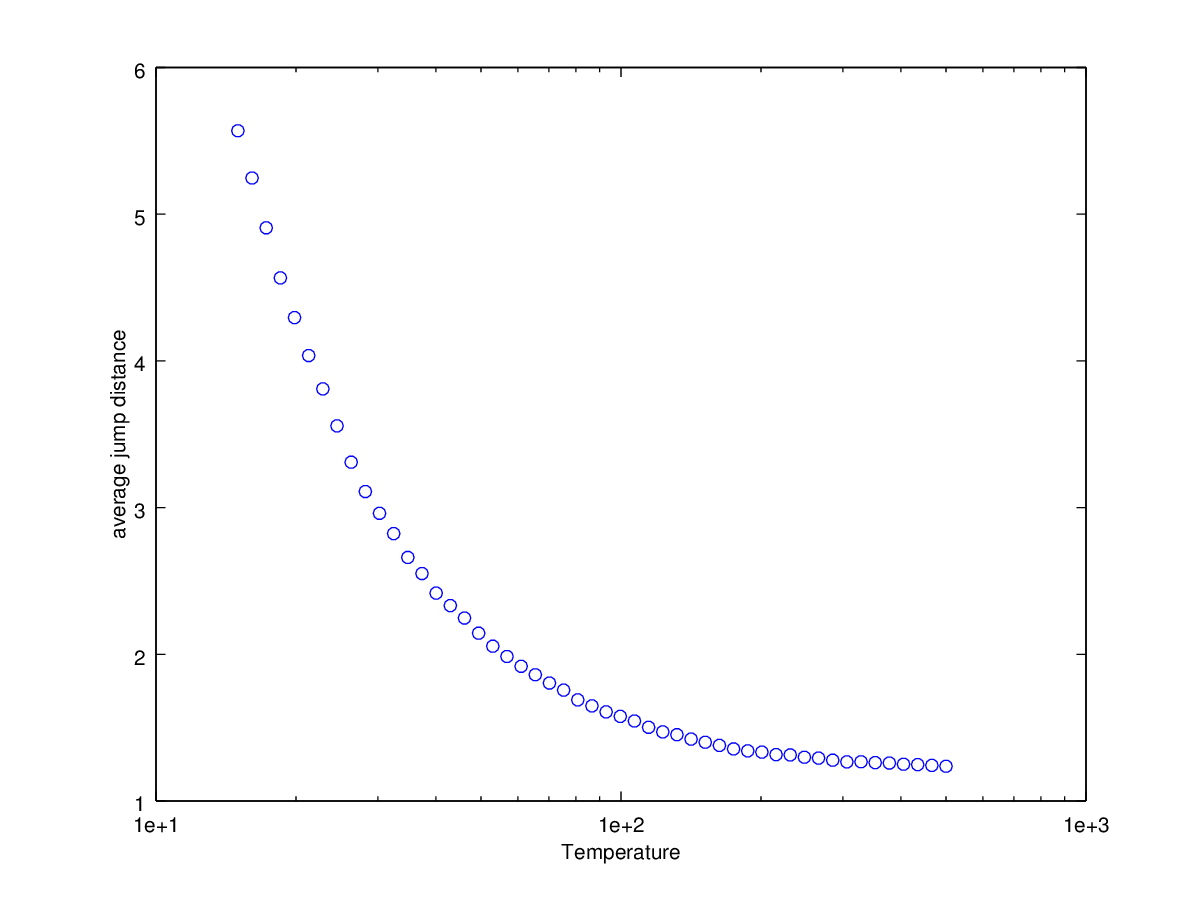
\includegraphics[scale=.50]{TvRGreat.png}
\caption{Temperature vs average jump distance .}
\label{TvsRbar}
\end{center}
\end{figure}

\begin{figure}[htbp]
\begin{center}
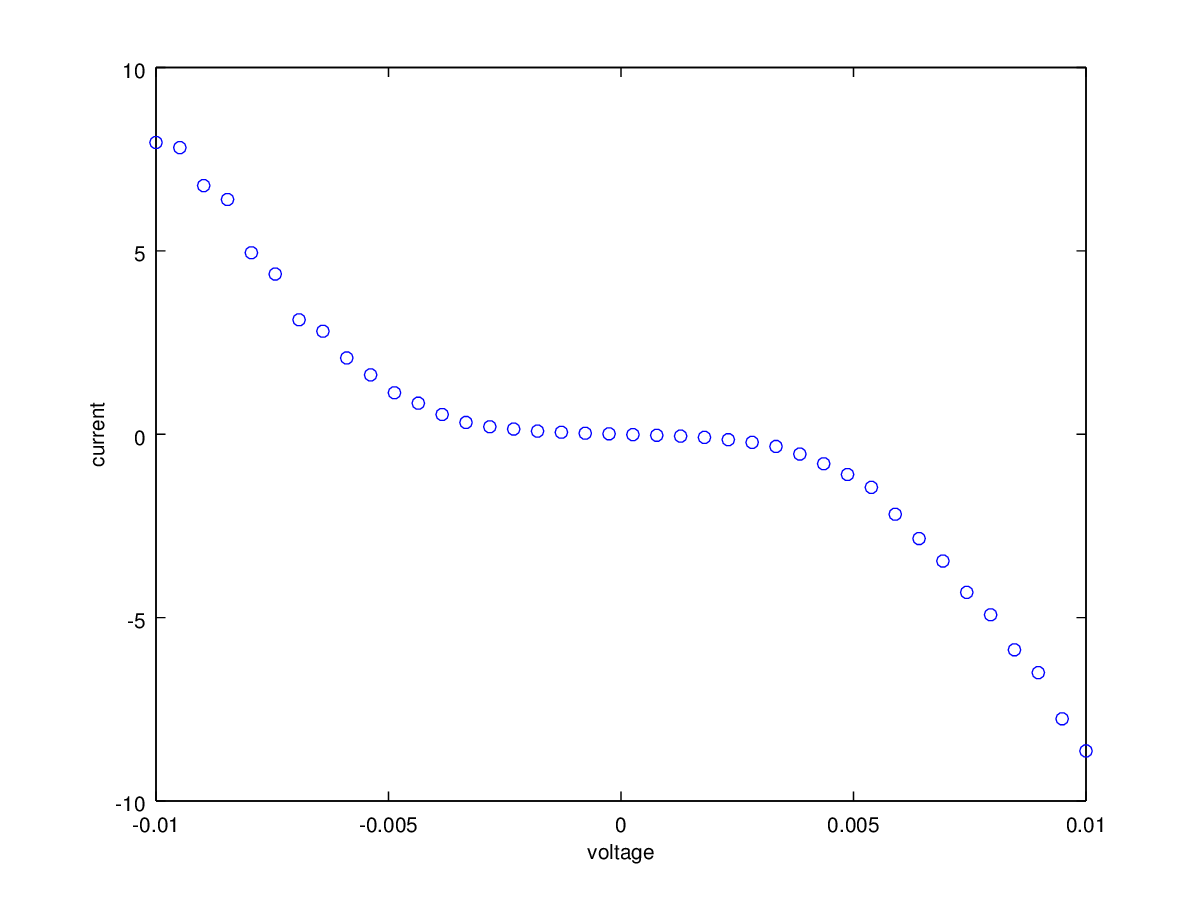
\includegraphics[scale=.50]{VvJGreat.png}
\caption{Current vs Voltage .}
\label{JvsV}
\end{center}
\end{figure}

\begin{figure}[htbp]
\begin{center}
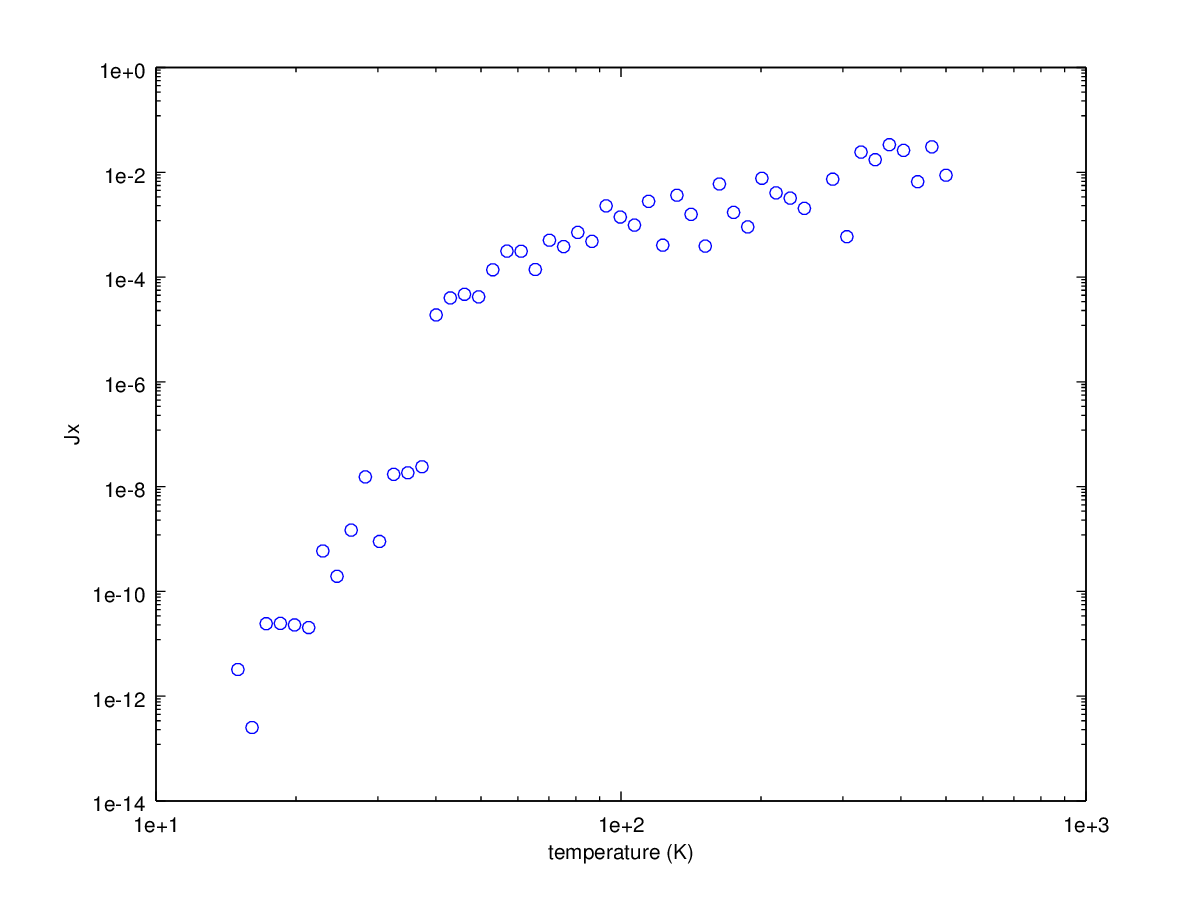
\includegraphics[scale=.50]{JvsT.png}
\caption{Temperature vs current .}
\label{TvJ}
\end{center}
\end{figure}


\begin{figure}[htbp]
\begin{center}
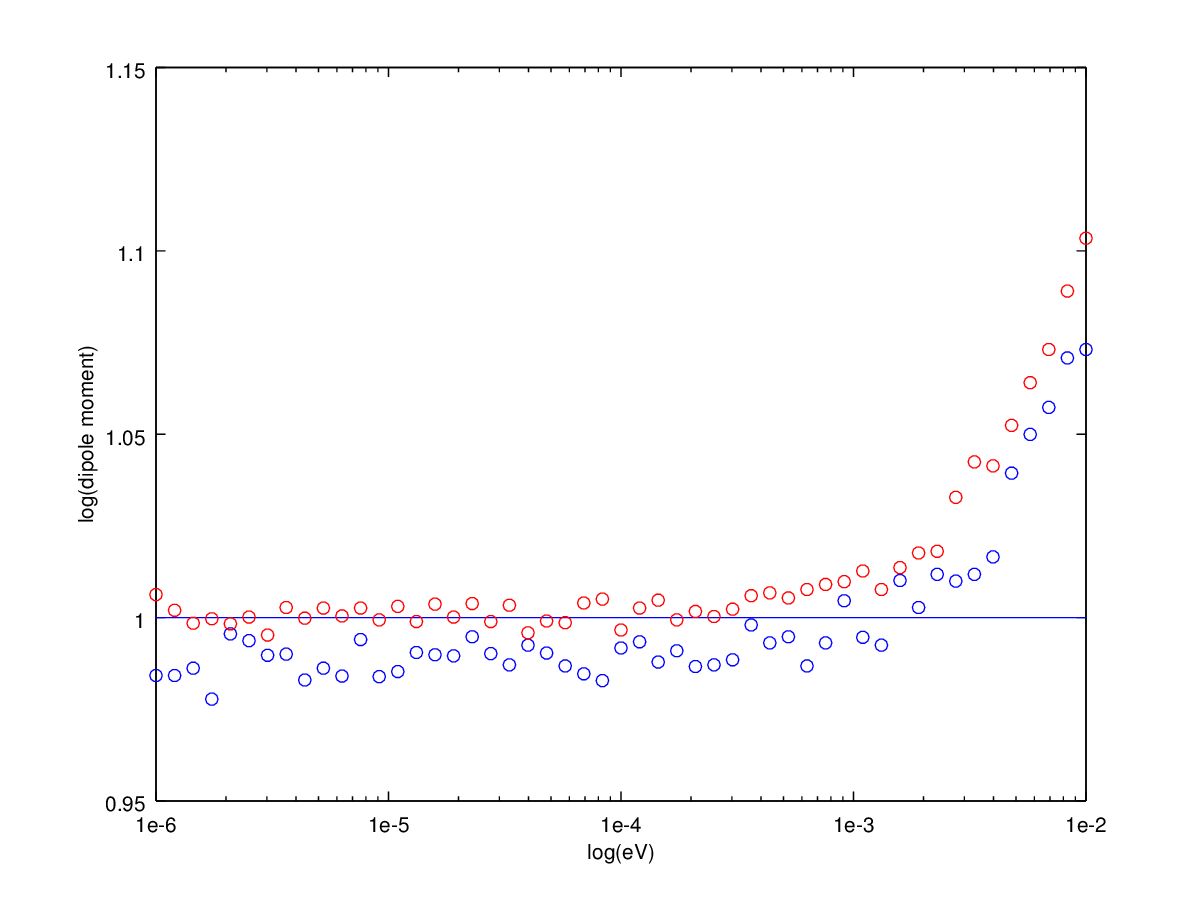
\includegraphics[scale=.50]{VoltageVsDipole.png}
\caption{This is a plot of the voltage vs the dipole moment of the electrons. The red dots are for a system without a temperature gradient. The blue dots are for a system with a temperature gradient. When the dipole moment becomes 0, the thermal force is pushing with as much strength aas the electric force. Using the Seebeck equation, we can estimate the Seebeck coefficient to be $10 \mu$}
\label{TvJ}
\end{center}
\end{figure}

